
\documentclass[12pt]{article}

\usepackage[utf8]{inputenc}
\usepackage[greek, english]{babel}

% Packages
\usepackage{MnSymbol}
\usepackage{alphabeta}
\usepackage{amsfonts}
\usepackage{amsmath}
\usepackage{amsthm}
\usepackage{caption}
\usepackage{graphicx}
\usepackage{latexsym}
\usepackage{stackrel}
\usepackage{titlesec}

% Commands
\newcommand{\R}{\mathbb{R}}
\newcommand{\N}{\mathbb{N}}
\newcommand{\norm}[1]{\left\lVert#1\right\rVert}
\newcommand{\margin}{\hspace{4pt}}
\newcommand{\centered}[1]{\begin{align*}#1\end{align*}}
\newcommand{\plot}{\includegraphics}

% Environments
\newenvironment{rcases}
	{\left.\begin{aligned}}
	{\end{aligned}\right\rbrace}

\newenvironment{matlab}
	{\begin{figure}[hp]\centering\captionsetup{justification=centering}}
	{\end{figure}}

\setlength{\parindent}{0in}
\setlength{\oddsidemargin}{0in}
\setlength{\textwidth}{6.5in}
\setlength{\textheight}{10in}
\setlength{\topmargin}{-1.0in}
\setlength{\headheight}{18pt}

\titlespacing*{\subsection}
{0pt}{5.5ex plus 1ex minus .2ex}{4.3ex plus .2ex}

\title{\hugeΑλγοριθμική Επιχειρησιακή Έρευνα\\Δεύτερη Εργασία}
\author{Σιώρος Βασίλειος\\Ανδρινοπούλου Χριστίνα}
\date{Οκτώβριος 2019}

\begin{document}

\maketitle

\pagenumbering{gobble}

\pagebreak


\subsection*{1. Find a differentiable function \( f: \R \rightarrow \R \) such that f does not have an extremum at its
critical point.}

Έστω η συνάρτηση \( f(x) = x^3 : \R \rightarrow \R \), η οποία είναι γνωστό ότι είναι
παραγωγίσιμη στο \( \R \). στο σημείο λόγους σαφήνειας, θα αποδείξουμε τη συνέχεια και την παραγωγισιμότητα της
στο \( x = 0 \). \\

\( \bullet \) \textbf{Συνέχεια:} \\

\begin{align*}
    &\begin{rcases}
        \lim_{x \to 0^-} f(x) & = \lim_{x \to 0^-} x^3 & = 0 \\
        \lim_{x \to 0^+} f(x) & = \lim_{x \to 0^+} x^3 & = 0
    \end{rcases}
    \Rightarrow \\
    &\lim_{x \to 0} f(x) = 0
\end{align*}

\begin{align*}
    &\begin{rcases}
        f(0) = 0^3 & = 0 \\
        \lim_{x \to 0} f(x) & = 0
    \end{rcases}
    \Rightarrow \\
    &f(0) = \lim_{x \to 0} f(x)
\end{align*}

\( \bullet \) \textbf{Παραγωγισιμότητα:} \\

\begin{align*}
    &\begin{rcases}
        \lim_{x \to 0^-} \frac{f(x) - f(0)}{x - 0} &= \lim_{x \to 0^-} \frac{x^3}{x} &= \lim_{x \to 0^-} x^2 &= 0 \\
        \lim_{x \to 0^+} \frac{f(x) - f(0)}{x - 0} &= \lim_{x \to 0^+} \frac{x^3}{x} &= \lim_{x \to 0^+} x^2 &= 0
    \end{rcases}
    \Rightarrow \\
    &\lim_{x \to 0} \frac{f(x) - f(0)}{x - 0} = 0
\end{align*} \\

Επομένως, δείξαμε ότι η συνάρτηση \( f(x) = x^3 \) είναι συνεχής και παραγωγίσιμη στο σημείο \( x = 0 \). \\

Το σημείο \( x = 0 \) αποτελεί κρίσιμο σημείο της \(f\), αφού η παράγωγός της μηδενίζεται εκεί.
Ωστόσο, όπως φαίνεται και από την ακόλουθη γραφική παράσταση, το σημείο \( x = 0 \)  δεν αποτελεί ακρότατο της. \\

\pagebreak

\begin{matlab}
    \plot{cubic_figure}
    \caption{An example of a differentiable function \( f: \R \rightarrow \R \) which does not have an extremum at its critical point}
\end{matlab}

\vspace{2in}

\pagebreak

\subsection*{2. Given a positive integer \( S \), which decompositions
\centered{a_1 + \dotsb + a_n = S}
with the \( a_i \) positive integers have the largest product \( a_1 \cdot \dotsb \cdot a_n \)?}

Αρχικά, μοντελοποιήσαμε το πρόβλημα, με στόχο να αναδείξουμε κάποιο πιθανό μοτίβο. \\

Παρατίθονται τα ευρήματα μας, όσον αφορά ακέραιες τιμές στο διάστημα \( \lbrack 10, \margin 20 \rbrack \). \\

\centered{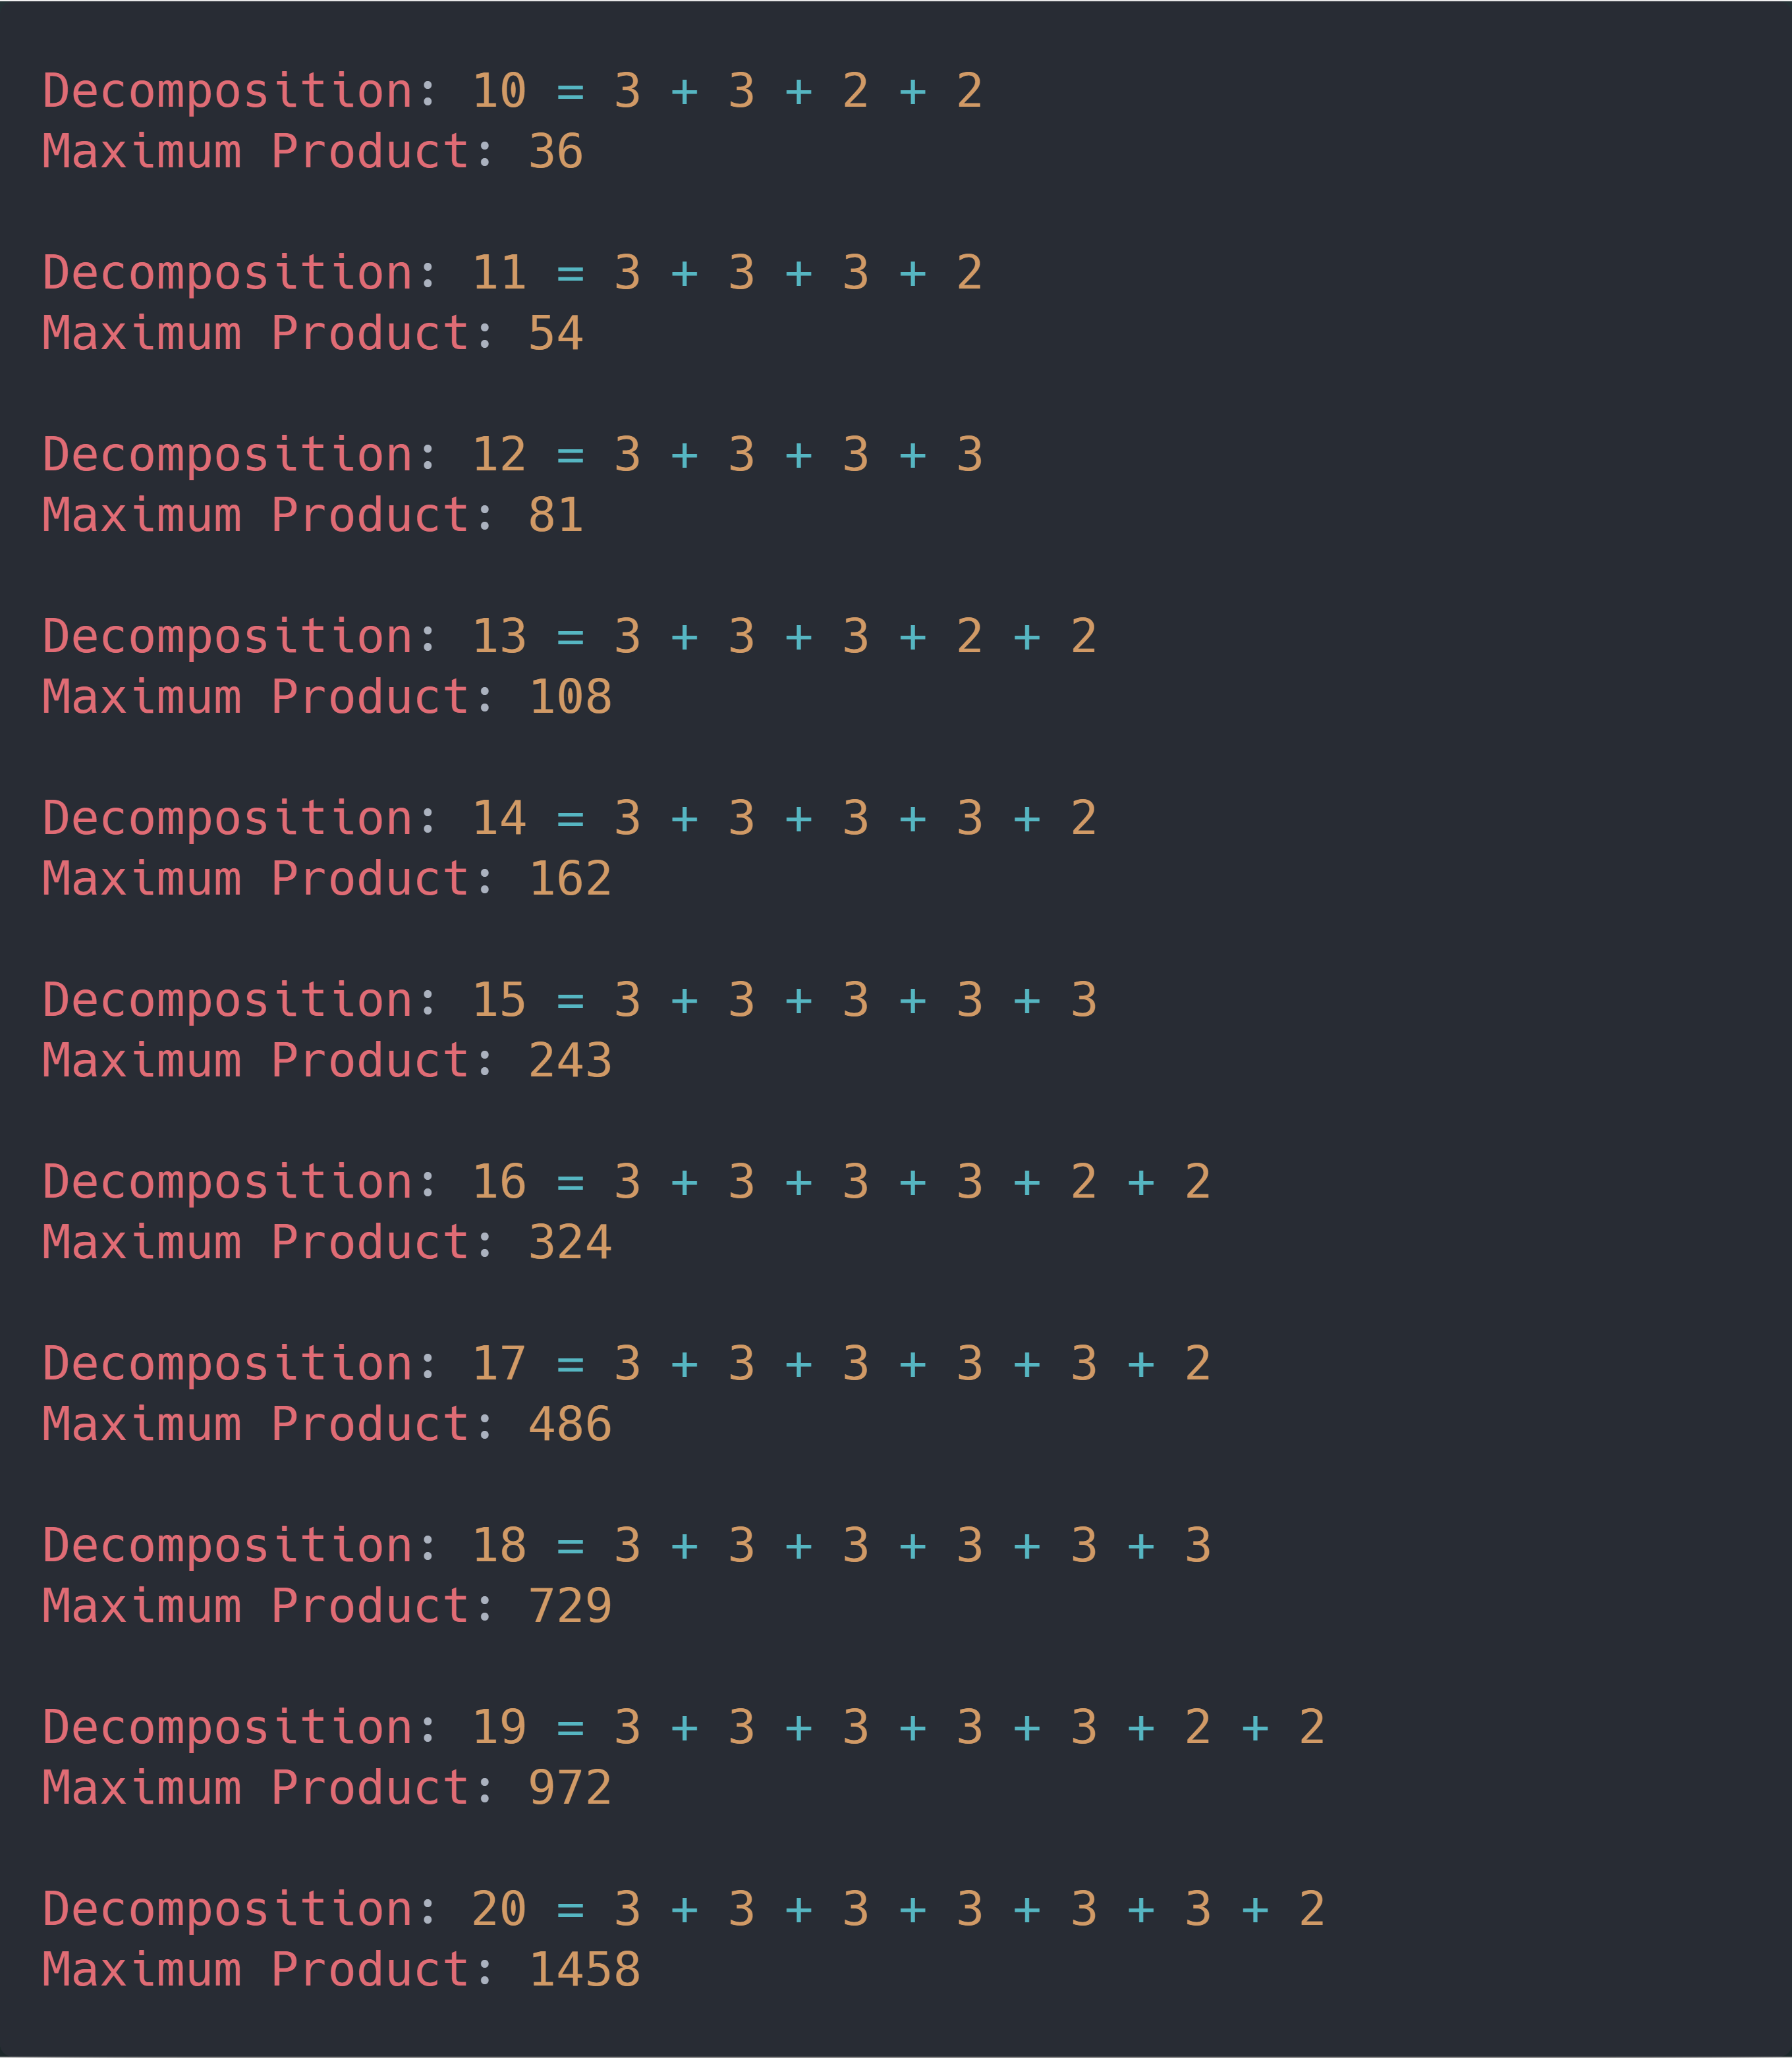
\includegraphics[scale=0.171875]{partition_output.png}} \\

Παρατηρούμε πως, σε κάθε περίπτωση, η αποδόμηση του εκάστοτε αριθμού με το μέγιστο γινόμενο αποτελείται αποκλειστικά από 3 και 2. \\

Θεωρούμε τυχαίο θετικό ακέραιο \( S \) και την αποδόμησή του \\

\centered{S = a_1 + \dotsb + a_n}

με το μέγιστο γινόμενο \\

\centered{\stackrel{max}{\prod} = \prod_{i = 1}^{n} a_i}

Έστω ότι υπάρχει \( 1 \leq k \leq n \) τέτοιο ώστε \( a_k \geq 4 \).
Διακρίνουμε τις εξής περιπτώσεις: \\

\( \bullet \) \( a_k = 2 \cdot l \margin \mid \margin l \in \N^+ \) \\

Δεδομένου ότι \( a_k \geq 4 \), έχουμε

\begin{align*}
    &\begin{rcases}
        a_k & & \geq 4 & \Leftrightarrow a_k & \geq 0 \\
        a_k & & \geq 4 & \Leftrightarrow a_k - 4 & \geq 0
    \end{rcases}
    \stackrel{\times}{\Rightarrow} \\
    &a_k \cdot (a_k - 4) \geq 0 && \Leftrightarrow \\
    &a_k^2 - 4 \cdot a_k \geq 0 && \Leftrightarrow \\
    &a_k^2 \geq 4 \cdot a_k && \Leftrightarrow \\
    &\frac{a_k^2}{4} \geq a_k
\end{align*}

Δεδομένου ότι

\centered{a_k = 2 \cdot l \margin \mid \margin l \in \N^+ \Leftrightarrow a_k \in N^+}

μπορούμε να ορίσουμε μια νέα αποδόμηση του \( S \), ως εξής

\centered{S = a_1 + \dotsb + \frac{a_k}{2} + \frac{a_k}{2} + \dotsb + a_n}

Το γινόμενο της παραπάνω αποδόμησης είναι

\begin{align*}
    \prod_{i = 1}^{n} a_i & = a_1 \times \dotsb \times \frac{a_k}{2} \times \frac{a_k}{2} \times \dotsb \times a_n && \Leftrightarrow \\
    \prod_{i = 1}^{n} a_i & = a_1 \times \dotsb \times \frac{a_k^2}{4} \times \dotsb \times a_n && \Leftrightarrow \\
    \prod_{i = 1}^{n} a_i & \geq a_1 \times \dotsb \times a_k \times \dotsb \times a_n && \Leftrightarrow \\
    \prod_{i = 1}^{n} a_i & \geq \stackrel{max}{\prod}
\end{align*}

Το παραπάνω αποτέλεσμα είναι αδύνατον, αφού υποθέσαμε πως \( \stackrel{max}{\prod} \) είναι η αποδόμηση του θετικού ακεραίου
\( S \) με το μέγιστο γινόμενο. Καταλήξαμε δηλαδή σε άτοπο, γεγονός που συνεπάγεται ότι η υπόθεση μας ήταν λανθασμένη. \\

Ως εκ τούτου δεν υπάρχει \( 1 \leq k \leq n \) τέτοιο ώστε \( a_k \geq 4 \). \\

\( \bullet \) \( a_k = 2 \cdot l + 1 \margin \mid \margin l \in \N \) \\

Δεδομένου ότι \( a_k \geq 4 \), έχουμε

\centered{a_k = 2 \cdot l + 1 \geq 4 \Leftrightarrow l \geq 2}

και άρα

\begin{align*}
    &\begin{rcases}
        l & \geq 2 & \Leftrightarrow l & \geq 1 \\
        l & \geq 2 & \Leftrightarrow l - 1 & \geq 1 \\
    \end{rcases}
    \stackrel{\times}{\Rightarrow} \\
    &l \cdot (l - 1) & \geq 1 && \Leftrightarrow \\
    &l^2 - l & \geq 1 && \Leftrightarrow \\
    &l^2 - l + 2 \cdot l & \geq 1 + 2 \cdot l && \Leftrightarrow \\
    &l^2 + l & \geq 1 + 2 \cdot l && \Leftrightarrow \\
    &l \cdot (l + 1) & \geq 2 \cdot l + 1 && \Leftrightarrow \\
    &l \cdot (l + 1) & \geq a_k
\end{align*}

Δεδομένου ότι

\centered{l \in \N \cap l \geq 2 \Leftrightarrow l \in N^+}

μπορούμε να ορίσουμε μια νέα αποδόμηση του \( S \), ως εξής

\centered{S = a_1 + \dotsb + l + (l + 1) + \dotsb + a_n}

Το γινόμενο της παραπάνω αποδόμησης είναι

\begin{align*}
    \prod_{i = 1}^{n} a_i & = a_1 \times \dotsb \times l \times (l \times 1) \times \dotsb \times a_n && \Leftrightarrow \\
    \prod_{i = 1}^{n} a_i & \geq a_1 \times \dotsb \times a_k \times \dotsb \times a_n && \Leftrightarrow \\
    \prod_{i = 1}^{n} a_i & \geq \stackrel{max}{\prod}
\end{align*}

Το παραπάνω αποτέλεσμα είναι αδύνατον, αφού υποθέσαμε πως \( \stackrel{max}{\prod} \) είναι η αποδόμηση του θετικού ακεραίου
\( S \) με το μέγιστο γινόμενο. Καταλήξαμε δηλαδή σε άτοπο, γεγονός που συνεπάγεται ότι η υπόθεση μας ήταν λανθασμένη. \\

Ως εκ τούτου δεν υπάρχει \( 1 \leq k \leq n \) τέτοιο ώστε \( a_k \geq 4 \). \\

\pagebreak

Η μονάδα, όντας το ουδέτερο στοιχείου το πολλαπλασιασμού, δεν συνεισφέρει θετικά στο τελικό γινόμενο καμίας αποδόμησης
που την εμπεριέχει κι ως εκ τουτου δεν θα εμφανίζεται σε καμία αποδόμηση μεγίστου γινομένου, πλην τετριμμένων περιπτώσεων. \\

Από τα πειράματα μας παρατηρούμε πως, ο αριθμός 2 δεν εμφανίζεται παραπάνω από 2 φορές σε καμία αποδόμηση μεγίσου γινομένου. \\

Αυτό είναι λογικό καθώς, δεδομένης μίας αποδόμησης του θετικού ακεραίου \( S \) της μορφής

\centered{S = a_1 + \dotsb + 2 + 2 + 2 + \dotsb + a_n}

μπορούμε να ορίσουμε μία νέα αποδόμηση

\centered{S = a_1 + \dotsb + 3 + 3 + \dotsb + a_n}

της οποίας το γινόμενο είναι

\begin{align*}
    \prod_{i = 1}^{n} a_i & = a_1 \times \dotsb \times 3 \times 3 \times \dotsb \times a_n && \Leftrightarrow \\
    \prod_{i = 1}^{n} a_i & = a_1 \times \dotsb \times 9 \times \dotsb \times a_n && \Leftrightarrow \\
    \prod_{i = 1}^{n} a_i & \geq a_1 \times \dotsb \times 8 \times \dotsb \times a_n && \Leftrightarrow \\
    \prod_{i = 1}^{n} a_i & \geq a_1 \times \dotsb \times 2 \times 2 \times 2 \times \dotsb \times a_n
\end{align*}

Έτσι η αποδόμηση μεγίστου γινομένου δίνεται από τη σχέση

\centered{S = 3 \cdot x + 2 \cdot \frac{S - 3 \cdot x}{2}}

και το γινόμενο της από τη σχέση

\centered{\stackrel{max}{\prod} = 3^x \times 2^{\frac{S - 3 \cdot x}{2}}}

\vspace{2in}

\pagebreak

\subsection*{3. Find the optimal solution to the Diet Problem when the cost function is
\centered{Cost(x_1, x_2) = x_1 + x_2 \text{.}}}

Οι περιορισμοί μας είναι οι εξής

\begin{align*}
    30 \cdot x_1 + 5 \cdot x_2 & \geq 60 \\
    15 \cdot x_1 + 10 \cdot x_2 & \geq 70 \\
    x_1, x_2 & \geq 0
\end{align*}

και επιθυμούμε να ελαχιστοποιήσουμε τη συνάρτηση

\centered{Cost(x_1, x_2) = x_1 + x_2}

\begin{matlab}
    \plot{diet_problem_figure}
    \caption{The Optimal Solution to the Diet Problem when the total cost is given by the function \( Cost(x_1, x_2) = x_1 \cdot x_2 \)}
\end{matlab}

\pagebreak

Παρατηρούμε ότι, δεν ορίζεται ευθεία, η οποία αντιστοιχεί σε κόστος χαμηλότερο του \textbf{4.67}, τέτοια ώστε,
έστω και ένα σημείο της να πληροί κάθε περιορισμό. Ως εκ τούτου το σημείο τομής των ευθειών

\begin{align*}
    15 \cdot x_1 + 10 \cdot x_2 & = 70 \\
    x_2 & = 0
\end{align*}

δηλαδή το σημείο \textbf{(4.67, 0)}, αποτελεί τη βέλτιστη λύση.

\vspace{2in}

\pagebreak

\subsection*{4. Let A,B Rnn. Show that the traditional way of computing their product AB requires
a total of (2n 1)n2 arithmetic operations.}

\vspace{2in}

\pagebreak

\subsection*{5. Consider the problem of solving a system of n linear equations in n unknowns. Show
that the Gaussian elimination method requires O(n3) arithmetic operations in order to either
compute a solution or to decide that no solution exist.}

\vspace{2in}

\pagebreak

\subsection*{6. Suppose that we are given a set of vectors in Rn that form a basis and let y be an
arbitrary vector in Rn. We wish to express y as a linear combination of the basis vectors. How
can this by accomplished?}

\vspace{2in}

\pagebreak

\subsection*{7. Study the paper with title: Do dogs know Calculus? found in the Readings folder.}

\vspace{2in}

\pagebreak

\end{document}
